% Arshad Ansari
\documentclass[12pt]{article}
\usepackage{fontspec}
\usepackage{polyglossia}
\usepackage[T1]{fontenc}
%\usepackage{fontenc}
\usepackage[utf8]{inputenc}
\usepackage{anyfontsize}
\usepackage{mathptmx}
\usepackage{graphicx}
\usepackage[margin=3cm]{geometry}
\usepackage{mdwlist}
\usepackage{longtable}
\usepackage{mathtools}
\usepackage{float}
\usepackage{ragged2e}
\usepackage[backend=biber]{biblatex}
\addbibresource{report.bib}

\newfontfamily\englishfont{Times New Roman}
\newfontfamily\devanagarifont[Script=Devanagari]{Lohit Devanagari}

\graphicspath{ {figures/} }

\restylefloat{figure}

\setmainlanguage{english}
\setotherlanguages{sanskrit}

\begin{document}
\pagenumbering{gobble}
\newgeometry{left=3cm,top=2cm, bottom=0.1cm}
% Front Cover page
\thispagestyle{empty}

\begin{center}
  	\fontsize{16}{30}\selectfont DISSERTATION SYNOPSIS\\On\\
  	\fontsize{20}{30}\selectfont \textbf{'Sentiment Analysis of transliterated
        hindi and marathi script'}\\
  	\fontsize{14}{24}\selectfont Submitted in partial fulfillment of the
    requirements for the degree of\\
  	\fontsize{16}{30}\selectfont \textbf{Master of Engineering} in \textbf{Information Technology (AI and Robotics)} \\
  	\fontsize{16}{30}\selectfont By\\
  	\fontsize{16}{30}\selectfont \textbf{Mr. Mohammed Arshad Ansari}\\
    \fontsize{16}{30}\selectfont Under the guidance\\of\\\textbf{Prof. Sharvari Govilkar}\\(Asst. Prof. Computer Department)\\
	\vspace{30mm}
	\begin{figure}[ht!]
	  \centering
	  
\includegraphics[width=30mm]{piit.png}
	\end{figure}
  	\fontsize{14}{20}\selectfont \textbf{DEPARTMENT OF INFORMATION TECHNOLOGY\\PILLAI INSTITUTE OF INFORMATION TECHNOLOGY,\\
	ENGINEERING, MEDIA STUDIES \& RESEARCH\\ NEW PANVEL - 410206\\UNIVERSITY OF
    MUMBAI\\Academic Year 2015-16}

\end{center}

% Main page
\newpage
\begin{center}
  	\fontsize{14}{20}\selectfont \textbf{DEPARTMENT OF INFORMATION TECHNOLOGY\\PILLAI INSTITUTE OF INFORMATION TECHNOLOGY,\\
	ENGINEERING, MEDIA STUDIES \& RESEARCH\\ NEW PANVEL - 410206\\UNIVERSITY OF
    MUMBAI\\Academic Year 2015-16}

	\begin{figure}[ht!]
	  \centering
	  
\includegraphics[width=30mm]{piit.png}
	\end{figure}

  	\fontsize{12}{30}\selectfont \textbf{SYNOPSIS OF PROJECT WORK}\\
\end{center}
\begin{left}
    \begin{tabular}{ll}
        Name of the Dissertation: & Sentiment Analysis of transliterated hindi and marathi script\\
        \hfill&\hfill\\
        Student's Name: & Mr. Mohammed Arshad Ansari\\
        \hfill&\hfill\\
        Class: & M.E. (Information Technology)\\
        \hfill&\hfill\\
        College: & PIllai Institude of Information Technology, New Panvel\\
        \hfill&\hfill\\
        Semester: & IV\\
        \hfill&\hfill\\
        University Registration Number: & \\
        \hfill&\hfill\\
        Date of Registration: & \\
        \hfill&\hfill\\
        Exam Fee Receipt No.: & 12698\\
        \hfill&\hfill\\
        Name of Guide: & Prof. Sharvari Govilkar\\
        \hfill&\hfill\\
    \end{tabular}
\end{left}
\begin{left}
    \begin{tabular*}{\textwidth}{c @{\extracolsep{\fill}} ccc}
        \hfill&\hfill&\hfill\\
        \textbf{Semester}&\textbf{Exam Seat Number}&\textbf{Result (SGPI)}\\
        \hfill&\hfill&\hfill\\
        1st & 4651 & 7.00 \\
        \hfill&\hfill&\hfill\\
        2nd & 4501 & 6.14 \\ 
        \hfill&\hfill&\hfill\\
    \end{tabular*}
\end{left}


\restoregeometry

\pagenumbering{arabic}
\newpage
\begin{center}
  \vspace{30mm}
  \fontsize{24}{60}\selectfont \textbf{Abstract}\\
  \vspace{20mm}

    \fontsize{12}{20}\selectfont \justifying{There is a growing research on
        sentiment analysis of various languages, which is being supplanted
        heavily by those same techniques and methods being applied on the mix
        code or transliterated text for the same purpose. This growing research
        is a result of necessity created through the advent of social media as
        well as textual analysis of the data being collected online. This
        paper, rather than being a pioneer, is about extending that research
        for further improvement. Herein, we assess the existing status,
        standards and achievements of the researchers in the given field and
        supplant it with out proposed methology to increase precision.}\par\\
	\vspace{10mm}
    \fontsize{12}{20}\selectfont \justifying{Although, the current work is a
        proposal with improvements over established techniques, it is also
        however gonig to be quite comparative when it comes to the existing
        findings. The idea is to not just improve what has already been built
        or shown to be true, but also check if the simplest approach is still
        the best way to proceed or not. By this we mean the existing direct
        supervised learning for sentiment analysis, without much NLP or
        language specific work.}\par\\
	\vspace{10mm}
    \fontsize{12}{20}\selectfont \justifying{Since we shall be testing our
        approach against the existing state of the art as well as entering the
    area previously not under coverge (marathi transliterated text), this work
is bound to make great strides in the field of sentiment analysis.}\par\\


\end{center}


\section{Introduction}

\fontsize{12}{20}\selectfont Sentiment analysis is a process of analysing natural language and figuring out
the sentiments involved or expressed through the source material, with respect
to the topic. The basic idea behind sentiment analysis is that each textual
sentence may or may not contain some kind of polarity, expressing a degree of
emotions along with the information. It is much easier to read in to those
polarity when the text is spoken and not written due to the tone of the
speaker; whereas, in case of written text, it is the context that is useful
while determining the polarities in the statements. Sentiment analysis has
grown to be one of the most important research areas when it comes to textual
analysis on the web. Reason being, obviously, is to be able to make sense of
the data as well as to understand the tone of information being provided. There
are numerous application, ranging from product/customer support review to
improve quality of service (QOS) by corporations to understanding geo-political
motivations when certain news breaks. People react on social media, especially
when they are charged emotionally and when emotions take the form of textual
content to vent, it has been observed that it does in a manner which is more
close to a person's mother tongue.\\


\fontsize{12}{20}\selectfont Hindi is spoken by more than 500 million people around the world, making it one
of the most spoken language in the world. Besides, English has turned out to be
an international language, a lot of people speak English on the internet,
however; as described above, there are instances when people use english
language to phonetize and express in a foreign language. This is seen far more
in India subcontinent, where people prefer to write using english alphabets,
but most often, use the words from the mother tongue. If we only look at all
the youtube comments (especially if they are about some controversial issues),
we would see a lot of usage of such transliterated messages or mix-script
writing. Another behavior worth noting is related to vocabulary. People from
subcontinent use words such as 'Bye', 'Thank you', 'Good night', 'Please',
'Sorry' and intermix them with their native tongues. This mixture of language
has been observed profoundly at varying levels of society. Therefore, it would
not be very far-fetched to say that the languages are evolving by mixing
language themselves. This forms the necessary reason for why there needs to be
analysis of mixed-languages and it starts with analyzing that which is mostly
available, the mixed-script. Here, we are not going to invent something new,
nor are we going to do something entirely differently. However, the purpose
behind this work is to stand on the shoulders of giants and take the research
of what has already been done to what it can be. This we strive to do, by
improving the performances by innovatively applying techniques which have
worked better in other cases. Therefore, as it will be seen, our proposed
approach as well is a mixture of disparate attempts in varying domains (even
slightly) to come together for better whole.\\

\fontsize{12}{20}\selectfont Sentiment analysis is a lot tougher for languages that are outside eurozone,
due to their lexical syntax being very different from european languages as
well as due to majorly, less amount of work being done on it. Semantic analysis
requires annotated text corpus to train classifers, which is most of the time a
very huge manual task. It has been undertaken for English and for many other
European langauges, while at the same time, work from one supplementing work
for another language, due to the similarities existent in those languages. When
it comes to languages such as Hindi and Marathi, such resources are very less
compared to the above mentioned languages. Moreso for Marathi, since a lot of
work has been done and progress made in case of Hindi. Most of the reason for
the under development of the research for these languages are (1) Not much
annotated textual corpus needed for traning, (2) Lack of basic language tools
like taggers and parsers. These problems will be solved in time and this work
is a part of all the woks which will finally solve this problem. 
Having expressed the problem, in this work, we also laude the work that has
already gone in to this respective field, without which this would not have
been possible. It is really interesting to note, that a great amount of effort
has just started pouring in for this particular part of sentiment analysis. It
is naught with great anticipation that this work is being progressed. Besides,
as the sentiment analysis of the textual data being to shape more and more, the
greater the benefit will be to the field of general AI. When it comes to human
capacity, not representing emotions would be the biggest gap in the domain,
which exactly is sentiment analysis has started to fill. \\


\section{Literature Review}

\fontsize{12}{20}\selectfont Code mixing has been done for more than a couple decades and was investigated
during initial period by Gold \cite{gold_language_1967} for the purpose of
language identification. The same phenomenon for Indian langauges was worked
upon by Annamalai \cite{annamalai_anglicized_1978}, pioneering the research
field for the subcontinent languages. Recently, it was investigated by Elfarti
et. al. \cite{elfardy_token_2012} and was termed as linguistic code switching
by the research group. Karimi \cite{karimi_machine_2011} made the case for
machine translation for the purpose of transliteration in the survey and
suggested transliteration based on phoneme based approach and transliteration
generation using bilingual corpus, while presenting the key issues that arise
during the transliteration process. Dewaele \cite{dewaele_emotions_2010}
pointed out the strong emotional presence as being the main marker for the
existence of code switch that happens in textual corpus. Gupta et. al.
\cite{gupta_mining_2012} mined the tranlisteration pairs between hindi and
english from the music lyrics of bollywood songs for Fire'14 shared task, which
is quite handy for training in language sentiments. 

\fontsize{12}{20}\selectfont The issue of identification of language of the code - mix script is another
challenge that has been answered by the research community. A statistical
approach was proposed by Kundu and Chandra et. al. \cite{kundu_automatic_2012}
for the automatic detection of English words in Bengali + English (Benglish)
text. A conditional random field model for weakly supervised learning model was
used for word/token labelling by King and Abney \cite{king_labeling_2013} with
a good result of > 90\%. Barman \cite{barman_code_2014} used facebook user data
for identifying the language in mixed script and concluded that the supervised
learning outperforms the dictionary based approaches. POS Tagging and
transliteration efforts for Hindi + English data on social media was
experimented upon by Vyas et. al. \cite{vyas_pos_2014} and came to the
conclusion that any operation on transliteration text will largely benefit from
pos tagging. 

\fontsize{12}{20}\selectfont Although sentiment analysis is being worked upon for quite some time now and it
has already entered the mainstream application. There are works being done
transliteration of Indian languages, out of which some have been listed below
under this section.\\

\fontsize{12}{20}\selectfont Joshi et.al. \cite{joshi_fall-back_2010} performed experiment to compare three
approaches for the sentiment analysis of hindi text and found that HSWN
performs better than Machine Translation approach but under performs in
language traning of sentiment corpus in hindi. This was, however; performed in
2010 and the HSWN has been continually improving past these experiments. The
same result was reiterated with by Balamurali et. al.
\cite{hutchison_lost_2013}. Kashyap \cite{kashyap_hindi_????} found a way to
perform Hindi Word Sense Disambiguation using wordnet with encouraging results
for nouns. Subjective lexical resource was developed by Bakliwal et. al.
\cite{bakliwal_hindi_2012} by using only wordnet and graph traversal algorithm
for adverbs and adjectives.\\

\fontsize{12}{20}\selectfont Balamurali A R et. al. \cite{balamurali_a_r_cross-lingual_????} performed
experiement to figure out in language supervised training of sentiments against
the machine translated source for sentiment analysis. They found that the MT
based approach under performs much worse compared to in language traning of
sentiment. Fuzzy Logic membership function was used to determine the degree of
polarity of the sentiment for a given POS tagged preposition by Rana
\cite{shweta_rana_sentiment_2014}. Hindi Senti WordNet was developed by
Balamurali A. R. et. al. \cite{balamurali_a_r_cross-lingual_????} using the Senti Wordnet by using linked wordnet. HSWN along with negetion discourse was applied by Pandey
\cite{pandey_framework_2015} and Mittal et. al. \cite{mittal_sentiment_2013} or
sentiment analysis of Hindi language text corpora, with the accuracy of 80.21
achived. \\

\fontsize{12}{20}\selectfont There is only one work done on the sentiment analysis of hindi transliteration
by Srinivas (\cite{sharma_text_2015} and \cite{shashank_sharma_sentiment_????}
) and the approach taken was to tag words with identified language and then run
against respective POS tagger for languages and sentiment analysis done on the
output. The approach yielded 85\% percision. Although not much has been done on
marathi front, however; it is still in the works and pipeline.\\

\section{Problem Statement}

\fontsize{12}{20}\selectfont \textit{The proposed work is geared towards the problem of sentiment analysis
    of code - mix script (Romanized) for languages such as hindi and marathi.
    The current literature has brought the accuracy up to 85 percent for hindi
    transliterated text, which this work aims to take to 90-95 percent accuracy
    and paritially accomplish for marathi language as well.}



\section{Methodology}

\subsection{Scope of work}

\fontsize{12}{20}\selectfont The current word considers hindi/marathi text in romanized script as input
which may contain phonetic words, sounds; however, it is not considering social
language like gr8, rt, f9, etc as input source. For now it is considered as
noise for the result of this work. Although, we are not performing sentiment
analysis on English text as part of this text, which is simply because it has
been under taken in many works preceeding this one. Therefore, concentration
will solely be on the text which is transliterated hindi or marathi. Also, the
architecture of proposed approach has intergration in mind and hence, it will
be able to plug social sentiment analysis or twitter sentiment analysis or
plain english analysis and will work only for the transliterated text, while
taking inputs from the mentioned analyzers for their established polarity. The
results can be merged and shown to have improved the overall accuracy. 

\subsection{Proposed Approach}

\fontsize{12}{20}\selectfont There are going to me multiple approach for testing to be implemented as part
of this work. The purpose of those work will be to ensure that the proposed
system performs better than what has been accomplished by other researchers.
Although, here we will only go into the actual proposed system to understand
its working and predict the possible improvements.\\
The proposed approach we are to take in this work comprises of extending the
work of Srinivas \cite{shashank_sharma_sentiment_????} with multiple
improvement points at multiple level of the process. Each step is listed below
with the improvement suggested from this work. All the work done on that paper
has been uploaded to the website \cite{_linguistic_????}, which we shall be
using in this paper extensively and building on top of it. \\

\begin{figure}[ht!]
    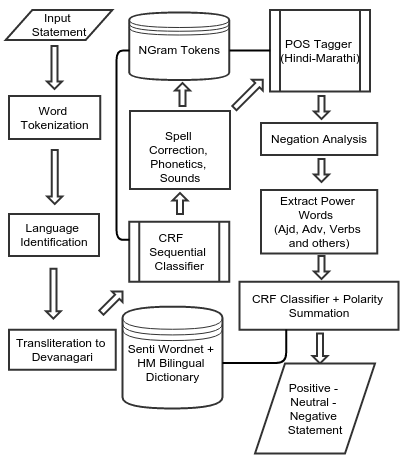
\includegraphics[width=140mm]{polarity-pickup.png}
    \caption{Flow diagram for the proposed approach}
\end{figure}


\subsubsection{Text Normalization}
\fontsize{12}{20}\selectfont Text normaliation step depends heavily on work of Srinivas
(\cite{sharma_text_2015}), which has following steps:
\begin{itemize*}
  \item \textbf{\textit{Language Identification}}; Tagging of the words as
      <word>/<tag>, where <tag> can be E or english, H for hindi and M or
      marathi,\\
  \item \textbf{\textit{Spelling Corrections}}; There are multipe ways to write
      Mujhe in hindi such as muze, muje, etc. To come to common and widely used
      spelling becomes very importnat\\
  \item \textbf{\textit{Ambiguous words}}; Words such as 'me' means same thing
      in english and marathi, where as in hindi it is sometimes used to say
      inside with another spelling being 'mein'. \\
  \item \textbf{\textit{Sounds}}; Words such as aww, oohh, ouch, ewww, etc.
      They do contain rich information when it comes to sentiments.\\
  \item \textbf{\textit{Phonetic words}}; Words such as pleej usually is
      misspelling of word please, spoken in some areas of the subcontinent. It
      gets written too in the similar manner.\\
  \item \textbf{\textit{Transliteration}}; Conversion of hindi/marathi words
      written in english to appropriate devnagari script.\\
\end{itemize*}

\fontsize{12}{20}\selectfont All then above enumerated steps have been covered by Srinivas
(\cite{sharma_text_2015}) and doesn't require us to go in the details of those,
however; we will look at some of those steps to get a proper grip on the
subject. At this point, this work will simply reuse those steps for hindi and try to
closely perform them for marathi as well. \\

\subsubsection{POS Tagging, Discourse analysis, Senti Word Net}
\fontsize{12}{20}\selectfont Before sentiment analysis can be performed, it is necessary to deal with few
important things. We are striving to extend and improve upon earlier work such
as Srinivas (\cite{sharma_text_2015}) and therefore following much in the same
footsteps. Both the step are explained further below.
Once we have the document in english or hindi, the next step is to run it
through POS tagger based on respective language. The approach will be straight
forward as detailed here \cite{vyas_pos_2014}. The POS Tagged prepositions
then shall be run through the negation discourse analysis to invert the POS
tagged adjectives and adverbs in case of negetive discourse as explained by Pandey
\cite{pandey_framework_2015} and Mittal et. al. \cite{mittal_sentiment_2013}.
The output of POS Tagger shall be used to look up sentiword identifier for the
word groups using Sentiwordnet or HSWN, for English and Hindi, respectively.
HSWN has been improved by Pandey \cite{pandey_framework_2015} by making
additions to it and that will be used in this work. Here, there are three major
improvements we are considering. Since, it was established
\cite{shashank_sharma_sentiment_????} that the basis for sentiment analysis
being POS tagged adjectives and adverbs gives much better result that depending
direcly on lexicon or wordnet look up for each work, we would be going that
route. Secondly, addition of discourse analysis would further enhance on the
existing work \cite{shashank_sharma_sentiment_????}.\\

\fontsize{12}{20}\selectfont Once we get sentiword identifier for each token - word, next step is to put it
through the classifier which will give the polartiy of the statement provided.
This polarity checking decision can be as simple as simple summation of all
word-token sentiment polarities or further analysis can be performed to figure
out what really is the polarity of word-token and its membership with negetive,
postive or neutral . This step being the vital one can be accomplished using
most trust classifier like SVM, Random Forests, however; impetus shall be given
on naive bayes classifier for brevity's sake. \\
\fontsize{12}{20}\selectfont Quite clearly, we have input as POS tagged statements with greater emphasis on
adjectives and adverbs that are inverted in case of negation present in the
preposition. Once we have this tagged information, we would like to test on
both the process of simple polarity count summation of the given input and
traning the classifier, in order to come up with the best possible result in
terms of accuracy. As can be seen in the figure, the classification uses
Senti Wordnet for polarity database, which is combination of HSWN and
Hindi-Marathi Bilingual Dictionary to match sentiments across language and to
look up is polarity.\\


\section{Requirement Analysis}

\begin{itemize*}
  \item \textbf{\textit{Hardware requirements}}; \\
      \hspace{20em}* i5 Processor\\
      \hspace{20em}* 8 GB Ram\\
      \hspace{20em}* 200 GB + HDD Space\\
      \hspace{20em}* Ubuntu OS 15.10\\

  \item \textbf{\textit{Software requiremetns and Tools}}; \\
      \hspace{20em}* Python 2.7\\
      \hspace{20em}* NLTK\\
      \hspace{20em}* Scikit Learn\\
      \hspace{20em}* Numpy\\

  \item \textbf{\textit{Data Requirment}}; \\
      \hspace{20em}* Code - Mix Data from Fire @ 2013 and 2014\\
      \hspace{20em}* Linugistic weebly data \cite{sharma_text_2015}\\


\end{itemize*}

\section{Conclusion}

\fontsize{12}{20}\selectfont The most important aspect of this work i.e. the results are what is coming
next. We will show that the approach proposed in this work performs better than
all the work presented here in literature, when considered independently. It is
the synergy, which the approach presented there, promises. The implementation
will happen for all ways that differ from the approach too, so that comparisons
can be made and conclusions drawn without the strawman arguments. \\

\fontsize{12}{20}\selectfont There is a lot of work to be performed before any concrete conclusion can be
expressed, however; There is a great possibility that the approach suggested in
the given work will result in improvement in the field of sentiment analysis,
that can again be extended for greater language coverage in as well as out of
indian languages. These strides towards such improvements will result in
machine's being able to understand human sentiments better, which is one of the
greatest challenge being faced by the research in general AI. Ours is but a
small step towards that goal. It will not be too far fetched to believe that
the improvements will range from 5 to 10 percent improvement where we will see
the accuracy reach 95 percent. \\



\printbibliography


\end{document}
